\documentclass[12pt,a4paper]{report}

% ============================================================================
% PACKAGES
% ============================================================================
\usepackage[utf8]{inputenc}
\usepackage[T1]{fontenc}
\usepackage{lmodern}
\usepackage[margin=1in]{geometry}
\usepackage{graphicx}
\usepackage{xcolor}
\usepackage{hyperref}
\usepackage{tikz}
\usepackage{longtable}
\usepackage{booktabs}
\usepackage{fancyhdr}
\usepackage{titlesec}
\usepackage{listings}
\usepackage{enumitem}

% TikZ Libraries
\usetikzlibrary{shapes.geometric, arrows.meta, positioning, fit, backgrounds}

% ============================================================================
% COLORS
% ============================================================================
\definecolor{primaryblue}{RGB}{26, 54, 93}
\definecolor{secondaryblue}{RGB}{59, 130, 246}
\definecolor{accentgreen}{RGB}{34, 197, 94}
\definecolor{warningorange}{RGB}{249, 115, 22}
\definecolor{lightgray}{RGB}{243, 244, 246}
\definecolor{darkgray}{RGB}{75, 85, 99}
\definecolor{chartblue}{RGB}{37, 99, 235}

% ============================================================================
% HYPERREF SETUP
% ============================================================================
\hypersetup{
    colorlinks=true,
    linkcolor=primaryblue,
    urlcolor=secondaryblue,
    pdftitle={EduX - Reports and Analytics Guide},
    pdfauthor={EduX Development Team},
}

% ============================================================================
% HEADER/FOOTER
% ============================================================================
\pagestyle{fancy}
\fancyhf{}
\fancyhead[L]{\textcolor{darkgray}{\small EduX School Management System}}
\fancyhead[R]{\textcolor{darkgray}{\small Reports Guide}}
\fancyfoot[C]{\textcolor{darkgray}{\thepage}}
\renewcommand{\headrulewidth}{0.4pt}

% ============================================================================
% TITLE FORMATTING
% ============================================================================
\titleformat{\chapter}[display]
  {\normalfont\huge\bfseries\color{primaryblue}}
  {\chaptertitlename\ \thechapter}{20pt}{\Huge}

\titleformat{\section}
  {\normalfont\Large\bfseries\color{primaryblue}}
  {\thesection}{1em}{}

\titleformat{\subsection}
  {\normalfont\large\bfseries\color{secondaryblue}}
  {\thesubsection}{1em}{}

% ============================================================================
% DOCUMENT
% ============================================================================
\begin{document}

% ----------------------------------------------------------------------------
% TITLE PAGE
% ----------------------------------------------------------------------------
\begin{titlepage}
    \centering
    \vspace*{2cm}
    
    {\Huge\bfseries\textcolor{primaryblue}{EduX}\par}
    \vspace{0.5cm}
    {\Large\textcolor{secondaryblue}{School Management System}\par}
    
    \vspace{2cm}
    
    
\begin{tikzpicture}
        \node[draw=primaryblue, line width=2pt, rounded corners=10pt, 
              minimum width=8cm, minimum height=3cm, fill=lightgray] 
              {\Huge\bfseries\textcolor{primaryblue}{Reports \& Analytics}};
    \end{tikzpicture}
    
    \vfill
    
    {\large\textcolor{darkgray}{Version 1.0}\par}
    {\large\textcolor{darkgray}{\today}\par}
\end{titlepage}

\tableofcontents
\newpage

% ============================================================================
% CHAPTER 1: DASHBOARD
% ============================================================================
\chapter{Dashboard Overview}

\section{Introduction}

The Dashboard provides a real-time overview of your school's key metrics, alerts, and quick actions.

\section{Dashboard Components}

\begin{center}
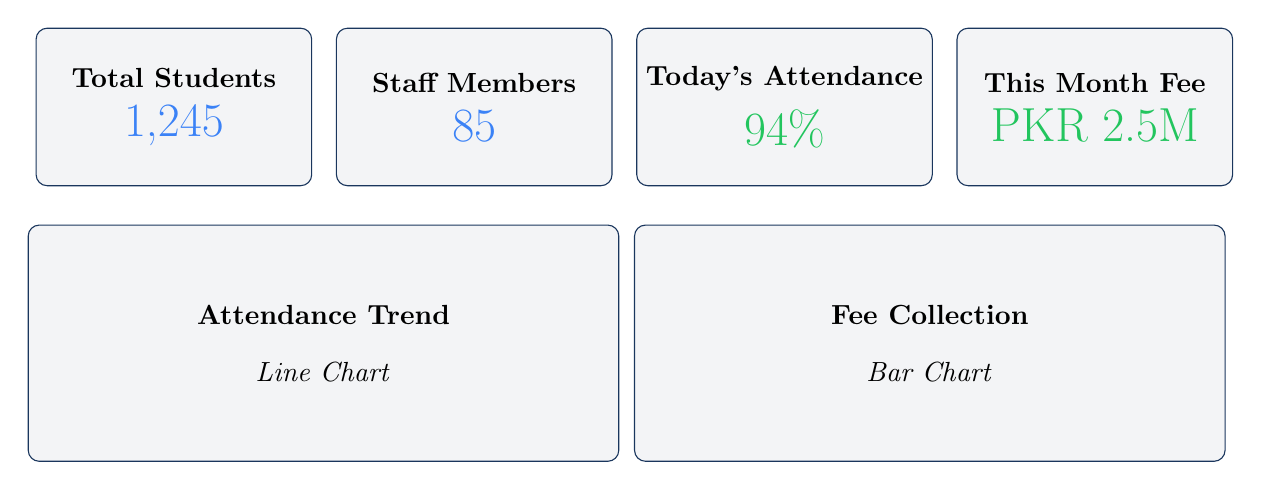
\begin{tikzpicture}[
    card/.style={draw=primaryblue, rounded corners, minimum width=3.5cm, 
                 minimum height=2cm, fill=lightgray, align=center}
]
    % Row 1 - Stats
    \node[card] (students) at (0,3) {
        \textbf{Total Students}\\[0.2cm]
        \textcolor{secondaryblue}{\LARGE 1,245}
    };
    \node[card, right=0.3cm of students] (staff) {
        \textbf{Staff Members}\\[0.2cm]
        \textcolor{secondaryblue}{\LARGE 85}
    };
    \node[card, right=0.3cm of staff] (attendance) {
        \textbf{Today's Attendance}\\[0.2cm]
        \textcolor{accentgreen}{\LARGE 94\%}
    };
    \node[card, right=0.3cm of attendance] (collection) {
        \textbf{This Month Fee}\\[0.2cm]
        \textcolor{accentgreen}{\LARGE PKR 2.5M}
    };
    
    % Row 2 - Charts placeholder
    \node[draw=primaryblue, rounded corners, minimum width=7.5cm, 
          minimum height=3cm, fill=lightgray, align=center] at (1.9,0) {
        \textbf{Attendance Trend}\\[0.3cm]
        \textit{Line Chart}
    };
    \node[draw=primaryblue, rounded corners, minimum width=7.5cm, 
          minimum height=3cm, fill=lightgray, align=center] at (9.6,0) {
        \textbf{Fee Collection}\\[0.3cm]
        \textit{Bar Chart}
    };
\end{tikzpicture}
\end{center}

\section{Key Metrics}

\begin{longtable}{@{}p{4cm}p{9cm}@{}}
\toprule
\textbf{Metric} & \textbf{Description} \\
\midrule
\endhead
Total Students & Active enrolled students \\
Staff Members & Active employees \\
Today's Attendance & Student attendance percentage \\
Fee Collection & Current month collection \\
Outstanding Fees & Total unpaid amounts \\
Defaulters & Students with overdue fees \\
Low Attendance & Students below 75\% attendance \\
\bottomrule
\end{longtable}

\section{Alerts Panel}

The dashboard shows important alerts:
\begin{itemize}[leftmargin=*]
    \item Low attendance students
    \item Fee defaulters
    \item Pending leave requests
    \item Upcoming exams
    \item System notifications
\end{itemize}

% ============================================================================
% CHAPTER 2: STUDENT REPORTS
% ============================================================================
\chapter{Student Reports}

\section{Available Reports}

\begin{longtable}{@{}p{4.5cm}p{8.5cm}@{}}
\toprule
\textbf{Report} & \textbf{Description} \\
\midrule
\endhead
Student Directory & Complete list with contact details \\
Class Strength & Students per class/section \\
Gender Distribution & Male/female ratio \\
New Admissions & Students admitted in period \\
Withdrawals & Students who left \\
Guardian Directory & Parent contact information \\
Birthday Report & Upcoming birthdays \\
\bottomrule
\end{longtable}

\section{Class Strength Chart}

\begin{center}
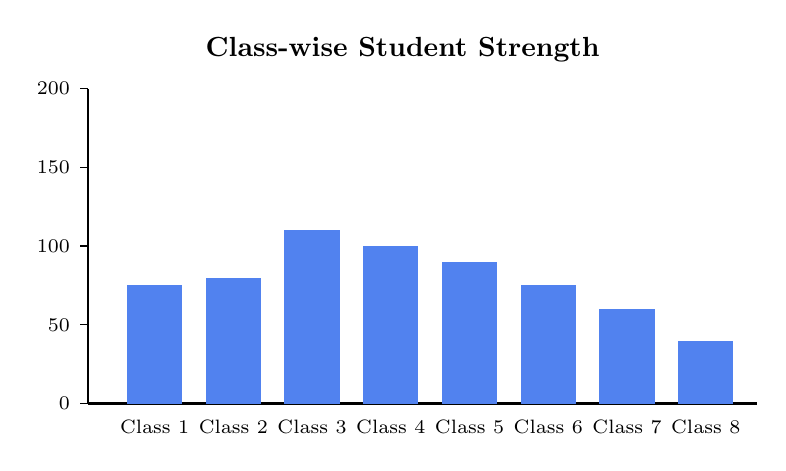
\begin{tikzpicture}
    % Title
    \node[font=\bfseries] at (4,4.5) {Class-wise Student Strength};
    
    % Y-axis
    \draw[thick] (0,0) -- (0,4);
    \foreach \y/\val in {0/0, 1/50, 2/100, 3/150, 4/200} {
        \draw (0,\y) -- (-0.1,\y) node[left, font=\scriptsize] {\val};
    }
    
    % X-axis
    \draw[thick] (0,0) -- (8.5,0);
    
    % Bars
    \fill[chartblue!80] (0.5,0) rectangle (1.2,1.5);
    \fill[chartblue!80] (1.5,0) rectangle (2.2,1.6);
    \fill[chartblue!80] (2.5,0) rectangle (3.2,2.2);
    \fill[chartblue!80] (3.5,0) rectangle (4.2,2.0);
    \fill[chartblue!80] (4.5,0) rectangle (5.2,1.8);
    \fill[chartblue!80] (5.5,0) rectangle (6.2,1.5);
    \fill[chartblue!80] (6.5,0) rectangle (7.2,1.2);
    \fill[chartblue!80] (7.5,0) rectangle (8.2,0.8);
    
    % Labels
    \foreach \x/\label in {0.85/1, 1.85/2, 2.85/3, 3.85/4, 4.85/5, 5.85/6, 6.85/7, 7.85/8} {
        \node[font=\scriptsize] at (\x,-0.3) {Class \label};
    }
\end{tikzpicture}
\end{center}

% ============================================================================
% CHAPTER 3: ATTENDANCE REPORTS
% ============================================================================
\chapter{Attendance Reports}

\section{Available Reports}

\begin{longtable}{@{}p{4.5cm}p{8.5cm}@{}}
\toprule
\textbf{Report} & \textbf{Description} \\
\midrule
\endhead
Daily Attendance & Date-wise attendance summary \\
Weekly Summary & Week-wise aggregation \\
Monthly Summary & Month-wise with trends \\
Student-wise & Individual attendance history \\
Class-wise & Section attendance comparison \\
Defaulters Report & Below threshold attendance \\
Staff Attendance & Employee attendance records \\
\bottomrule
\end{longtable}

\section{Attendance Trend}

\begin{center}
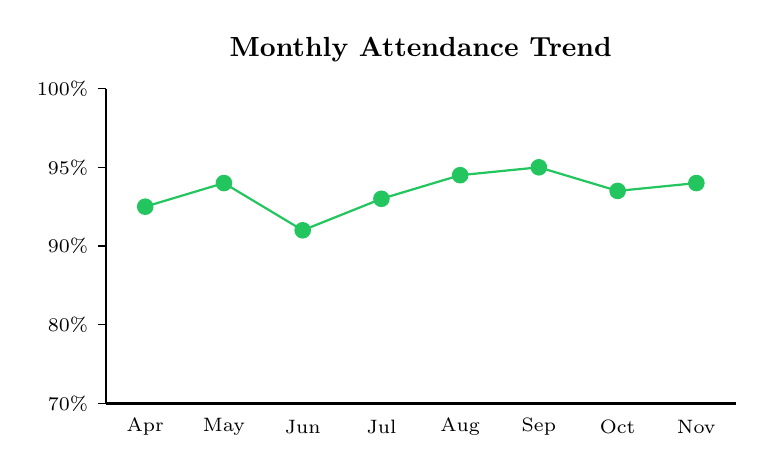
\begin{tikzpicture}
    % Title
    \node[font=\bfseries] at (4,4.5) {Monthly Attendance Trend};
    
    % Axes
    \draw[thick] (0,0) -- (0,4);
    \draw[thick] (0,0) -- (8,0);
    
    % Y-axis labels
    \foreach \y/\val in {0/70\%, 1/80\%, 2/90\%, 3/95\%, 4/100\%} {
        \draw (0,\y) -- (-0.1,\y) node[left, font=\scriptsize] {\val};
    }
    
    % X-axis labels
    \foreach \x/\month in {0.5/Apr, 1.5/May, 2.5/Jun, 3.5/Jul, 4.5/Aug, 5.5/Sep, 6.5/Oct, 7.5/Nov} {
        \node[font=\scriptsize] at (\x,-0.3) {\month};
    }
    
    % Line graph
    \draw[thick, accentgreen] 
        (0.5,2.5) -- (1.5,2.8) -- (2.5,2.2) -- (3.5,2.6) -- 
        (4.5,2.9) -- (5.5,3.0) -- (6.5,2.7) -- (7.5,2.8);
    
    % Points
    \foreach \x/\y in {0.5/2.5, 1.5/2.8, 2.5/2.2, 3.5/2.6, 4.5/2.9, 5.5/3.0, 6.5/2.7, 7.5/2.8} {
        \fill[accentgreen] (\x,\y) circle (3pt);
    }
\end{tikzpicture}
\end{center}

% ============================================================================
% CHAPTER 4: FEE REPORTS
% ============================================================================
\chapter{Fee Reports}

\section{Available Reports}

\begin{longtable}{@{}p{4.5cm}p{8.5cm}@{}}
\toprule
\textbf{Report} & \textbf{Description} \\
\midrule
\endhead
Collection Summary & Period-wise collections \\
Outstanding Report & All unpaid amounts \\
Defaulters List & Overdue invoices \\
Class-wise Collection & Per-class fee status \\
Payment Register & All transactions \\
Concession Report & Discounts applied \\
Daily Collection & Day-wise cash book \\
\bottomrule
\end{longtable}

\section{Fee Collection Summary}

\begin{center}
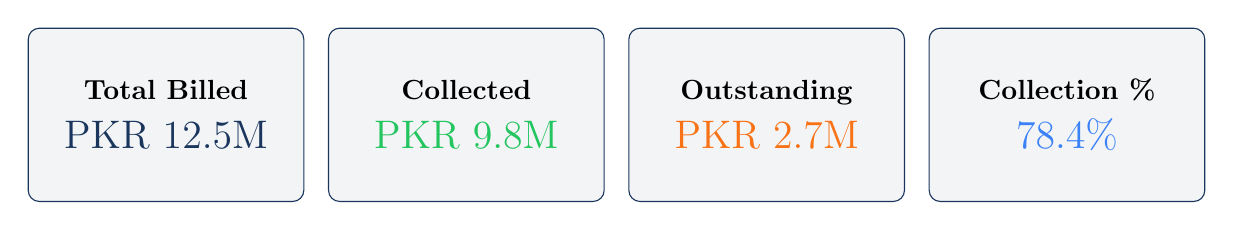
\begin{tikzpicture}[
    stat/.style={draw=primaryblue, rounded corners, minimum width=3.5cm, 
                 minimum height=2.2cm, fill=lightgray, align=center}
]
    \node[stat] (billed) at (0,0) {
        \textbf{Total Billed}\\[0.2cm]
        \textcolor{primaryblue}{\Large PKR 12.5M}
    };
    \node[stat, right=0.3cm of billed] (collected) {
        \textbf{Collected}\\[0.2cm]
        \textcolor{accentgreen}{\Large PKR 9.8M}
    };
    \node[stat, right=0.3cm of collected] (outstanding) {
        \textbf{Outstanding}\\[0.2cm]
        \textcolor{warningorange}{\Large PKR 2.7M}
    };
    \node[stat, right=0.3cm of outstanding] (percent) {
        \textbf{Collection \%}\\[0.2cm]
        \textcolor{secondaryblue}{\Large 78.4\%}
    };
\end{tikzpicture}
\end{center}

% ============================================================================
% CHAPTER 5: EXAM REPORTS
% ============================================================================
\chapter{Examination Reports}

\section{Available Reports}

\begin{longtable}{@{}p{4.5cm}p{8.5cm}@{}}
\toprule
\textbf{Report} & \textbf{Description} \\
\midrule
\endhead
Result Sheet & Complete marks listing \\
Grade Distribution & Students per grade \\
Toppers List & Rank-wise students \\
Subject Analysis & Performance by subject \\
Comparative Report & Across multiple exams \\
Failed Students & Non-passed students \\
Report Cards & Printable format \\
\bottomrule
\end{longtable}

\section{Grade Distribution}

\begin{center}
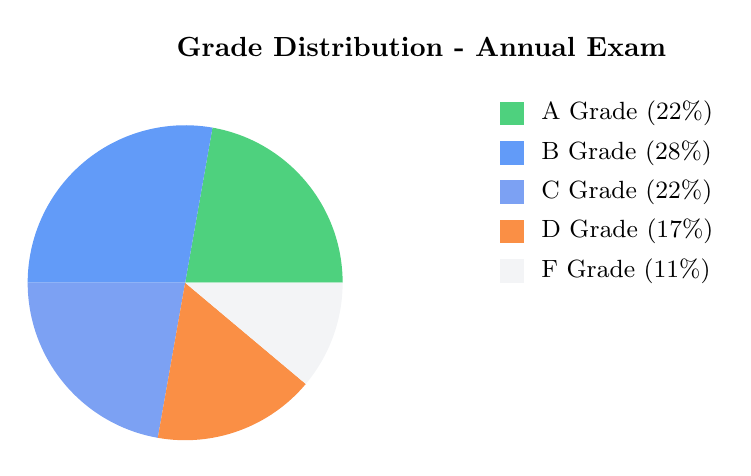
\begin{tikzpicture}
    % Title
    \node[font=\bfseries] at (3,3) {Grade Distribution - Annual Exam};
    
    % Pie chart simulation
    \fill[accentgreen!80] (0,0) -- (0:2) arc (0:80:2) -- cycle;
    \fill[secondaryblue!80] (0,0) -- (80:2) arc (80:180:2) -- cycle;
    \fill[chartblue!60] (0,0) -- (180:2) arc (180:260:2) -- cycle;
    \fill[warningorange!80] (0,0) -- (260:2) arc (260:320:2) -- cycle;
    \fill[lightgray] (0,0) -- (320:2) arc (320:360:2) -- cycle;
    
    % Legend
    \fill[accentgreen!80] (4,2) rectangle (4.3,2.3);
    \node[right, font=\small] at (4.4,2.15) {A Grade (22\%)};
    \fill[secondaryblue!80] (4,1.5) rectangle (4.3,1.8);
    \node[right, font=\small] at (4.4,1.65) {B Grade (28\%)};
    \fill[chartblue!60] (4,1) rectangle (4.3,1.3);
    \node[right, font=\small] at (4.4,1.15) {C Grade (22\%)};
    \fill[warningorange!80] (4,0.5) rectangle (4.3,0.8);
    \node[right, font=\small] at (4.4,0.65) {D Grade (17\%)};
    \fill[lightgray] (4,0) rectangle (4.3,0.3);
    \node[right, font=\small] at (4.4,0.15) {F Grade (11\%)};
\end{tikzpicture}
\end{center}

% ============================================================================
% CHAPTER 6: EXPORT OPTIONS
% ============================================================================
\chapter{Export Options}

\section{PDF Export}

PDF reports include:
\begin{itemize}[leftmargin=*]
    \item School header with logo
    \item Report title and date range
    \item Formatted data tables
    \item Charts and graphs
    \item Signature lines
    \item Page numbers
\end{itemize}

\section{Excel Export}

Excel exports provide:
\begin{itemize}[leftmargin=*]
    \item Raw data in tabular format
    \item Multiple sheets for complex reports
    \item Filter-ready columns
    \item Pivot table compatible
\end{itemize}

\section{Export Steps}

\begin{enumerate}[leftmargin=*]
    \item Navigate to desired report
    \item Apply filters (date range, class, etc.)
    \item Click \texttt{Export} button
    \item Select format (PDF / Excel)
    \item Choose save location
    \item Confirm export
\end{enumerate}

% ============================================================================
% CHAPTER 7: BACKUP & RESTORE
% ============================================================================
\chapter{Backup \& Restore}

\section{Creating Backups}

Navigate to \texttt{Settings} $\rightarrow$ \texttt{Backup}

\begin{enumerate}[leftmargin=*]
    \item Click \texttt{Create Backup}
    \item Enter description (optional)
    \item Choose location (local or external)
    \item Wait for backup completion
    \item Verify backup success
\end{enumerate}

\section{Automatic Backups}

Configure in Settings:
\begin{itemize}[leftmargin=*]
    \item Enable automatic backups
    \item Set frequency (daily/weekly)
    \item Set backup time
    \item Set retention period
    \item Set backup location
\end{itemize}

\section{Restoring Data}

\begin{enumerate}[leftmargin=*]
    \item Go to \texttt{Settings} $\rightarrow$ \texttt{Backup} $\rightarrow$ \texttt{Restore}
    \item Select backup file
    \item Review backup details
    \item Confirm restoration
    \item Restart application
\end{enumerate}

\textbf{Warning:} Restoring a backup will replace all current data.

\end{document}
